\documentclass[10pt,twocolumn]{article}

\usepackage[margin=0.75in]{geometry}
\usepackage{times}
\usepackage{graphicx}
\usepackage{booktabs}
\usepackage{amsmath,amssymb}
\usepackage{enumitem}
\usepackage{xcolor}
\usepackage{url}
\usepackage[numbers,sort&compress]{natbib}
\usepackage[hidelinks]{hyperref}
\usepackage{microtype}
\usepackage{caption}
\captionsetup{font=small,labelfont=bf,skip=4pt}
\setlength{\columnsep}{0.25in}
\setlength{\parskip}{0pt}
\setlist[itemize]{leftmargin=*,itemsep=1pt,topsep=2pt,parsep=0pt}
\setlist[enumerate]{leftmargin=*,itemsep=1pt,topsep=2pt,parsep=0pt}

\title{\vspace{-0.6em}Size Confounds Semantics:\\
An Audit of SING's Null-Space Leakage Score\vspace{-0.4em}}

\author{
Anonymous Authors\\
Workshop submission
}

\date{}

\begin{document}
\maketitle
\vspace{-1.2em}

\begin{abstract}
\vspace{-0.3em}
SING~\citep{sing2026} ranks classifiers by how much class-relevant semantics leak into the linear head's null space. Their reported standout is a ``DinoViT'' pretrained with DINO, which they find leaks least.
We checked that claim against public checkpoints and against size controls on the score itself.
Among public ViT-L/16 models that match SING's code or wrappers, every candidate is supervised or SWAG-supervised; none reproduces the reported 84.0\% top-1, and none is DINO.
Holding the architecture fixed, the absolute-shift score $|$AS$|$ grows by about a factor of $10$ as the removed null subspace expands from $d{=}24$ to $d{=}1048$ on ResNet50, ResNeXt101 and DINOv2-L. Matching the models at $d{=}24$ already disagrees with SING's published order (Kendall $\tau{=}0.29$).
A pooled log-linear fit of $|$AS$|$ against removed feature energy $\rho$ gives an exponent of $0.43$, close to the $\sqrt{\rho}$ geometric prediction, though separating energy from dimension remains incomplete.
We therefore also report a size-fair score $\mathrm{AS}_{\mathrm{fair}}$, which divides null removal by an energy-matched random-subspace baseline.
On all 13 SING models, $\mathrm{AS}_{\mathrm{SING}}$ recovers the published Fig.~6b ordering ($\tau{=}0.82$), while $\mathrm{AS}_{\mathrm{fair}}$ does not ($\tau{=}{-}0.18$), and two class-level claims reverse under bootstrap CIs.
Planted-leakage recovery is weak for both scores.
When null-space scores are used to compare architectures, we recommend reporting $\rho$ and $\mathrm{AS}_{\mathrm{fair}}$ alongside raw AS.
\vspace{-0.3em}
\end{abstract}

\section{Introduction}
\vspace{-0.2em}
A linear classifier on features $f\in\mathbb{R}^m$ has a null space of dimension $m{-}c$ (for $c$ classes) that leaves the logits unchanged.
SING~\citep{sing2026} treats class-relevant content in that null space as ``leakage'': material the head could have used, but did not.
Absolute Shift (AS) measures how far a CLIP-aligned~\citep{clip2021} translation of $f$ moves once the null component is stripped out. SING ranks 13 ImageNet models by AS (and by the IS/AS ratio) and singles out a ViT labeled ``DinoViT'' as the least leaky~\citep{dino2021}.

Related null-space tools appear in OOD detection~\citep{vim2022,cook2020} and overfitting scores~\citep{rezaei2023}.
Across architectures the null dimension $d{=}m{-}\mathrm{rank}(W)$ and the null energy fraction
$\rho = \mathbb{E}\|V_nV_n^\top f\|^2/\mathbb{E}\|f\|^2$
both swing by orders of magnitude.
If AS largely tracks how much energy is removed, then cross-model ``semantics'' rankings are partly rankings of null size.

\paragraph{What we find.}
SING's ``DinoViT'' is not identifiable as DINO: every matching public candidate is supervised, and none reproduces 84.0\% top-1.
Within-model AS$(d)$ curves rise by $\approx\!10\times$ from $d{=}24$ to $d{=}1048$ on ResNet50, ResNeXt101 and DINOv2-L; BiT~\citep{bit2020} is the exception, explained by translator cancellation.
Energy and dimension are hard to separate. A pooled fit yields exponent $a{=}0.43$ on $\rho$ against a $\sqrt{\rho}$ prediction of $0.5$, yet fixed-$\rho$ flatness is not clean.
On 13 models, size-fair $\mathrm{AS}_{\mathrm{fair}}$ breaks SING's published ranking ($\tau{:}\,0.82\to{-}0.18$) and reverses several claims, with the caveats below.
We treat $\mathrm{AS}_{\mathrm{fair}}$ as a reporting correction rather than a new leakage oracle.

\section{Background and the DinoViT identity}
\vspace{-0.2em}
\paragraph{SING AS in brief.}
Let $T(f)=Af+b$ be SING's released linear translator into CLIP space and $V_n$ an orthonormal basis of $\ker(W)$ (tolerance $10^{-5}$).
For a text direction $t$, SING's per-image absolute shift is the change in angle $\theta(T(f),t)$ after removing $V_nV_n^\top f$.
$\mathrm{AS}_{\mathrm{SING}}$ denotes the image-averaged $|$AS$|$ under full null removal (class text unless noted).

\paragraph{Exp~0b: ``DinoViT'' is not DINO.}
SING reports DinoViT at 84.0\% ImageNet top-1 (Supp.\ Table~2).
The released \texttt{models.yaml} loads a timm AugReg ViT-L/16; the supplement's wrapper uses torchvision ViT attribute names.
We ran five public ViT-L/16 candidates on the full 50k validation set (native and force-224):
torchvision IMAGENET1K\_V1 (79.67\%),
timm AugReg (85.85\%),
SWAG linear~\citep{swag2022} (85.14\%),
SWAG E2E (88.07\%),
and HF \texttt{google/vit-large-patch16-224} (81.98\%).
None lands in $84.0\pm0.3$ (Fig.~\ref{fig:exp0b}).
All five are supervised or SWAG weakly supervised. DINO never shipped a ViT-L with a 1000-way head~\citep{dino2021}.
So the DINO attribution in the headline result has no identifiable public checkpoint behind it.

\begin{figure}[t]
\centering
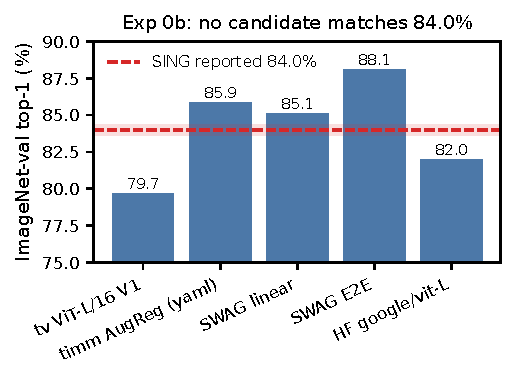
\includegraphics[width=\linewidth]{figs/fig_exp0b.pdf}
\vspace{-0.4em}
\caption{Exp~0b top-1 on ImageNet-val. No candidate matches SING's reported 84.0\%.}
\label{fig:exp0b}
\vspace{-0.6em}
\end{figure}

\paragraph{Exp~0 (re-analysis).}
Digitizing SING Supp.\ Fig.~6b IS/AS bars and correlating against measured null dimension gives Spearman $-0.46$ ($p{=}0.12$) over 13 models (DenseNet null dim $=27$ at tol $10^{-5}$).
Null energy is far more predictive: Spearman$(\rho_{\mathrm{full}},\mathrm{IS}/\mathrm{AS})={-}0.94$ ($p{=}1.9{\times}10^{-6}$).
DeiT3-L~\citep{deit3} has null dim $24$ yet the worst ratio, so dimension alone cannot explain the ranking. That is why we move to a within-model test.

\section{Within-model size dependence (Exp~1)}
\vspace{-0.2em}
We fix a 10k ImageNet-val subset (10 images/class) and remove random $d$-dimensional subspaces of each model's own null space ($d\in\{24,48,100,280,536,1048\}$, 20 seeds for $d{<}d_{\mathrm{null}}$) for ResNet50, ResNeXt101, BiT-R50x1 and DINOv2-L (all $d_{\mathrm{null}}{=}1048$), using SING's released translators.

\begin{figure}[t]
\centering
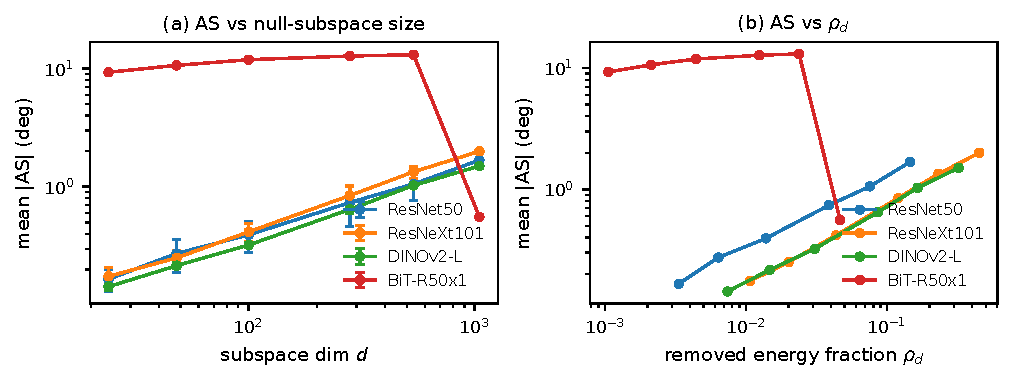
\includegraphics[width=\linewidth]{figs/fig_exp1_curves.pdf}
\vspace{-0.4em}
\caption{Exp~1: mean $|$AS$|$ vs.\ subspace size $d$ (a) and removed energy $\rho_d$ (b). BiT collapses at the full null (translator cancellation).}
\label{fig:exp1}
\vspace{-0.6em}
\end{figure}

\begin{table}[t]
\centering
\scriptsize
\setlength{\tabcolsep}{3pt}
\begin{tabular}{@{}lcccc@{}}
\toprule
Model & $r$ & $2\sigma$ band & $R^2$ vs $d$ & $R^2$ vs $\rho_d$ \\
\midrule
ResNet50   & 10.15 & $[5.83,14.48]$ & 0.983 & 0.983 \\
ResNeXt101 & 11.44 & $[6.93,15.95]$ & 0.977 & 0.977 \\
DINOv2-L   & 10.48 & $[8.85,12.10]$ & 0.974 & 0.974 \\
BiT-R50x1  & 0.060 & $[0.057,0.063]$ & 0.512 & 0.512 \\
\bottomrule
\end{tabular}
\vspace{-0.4em}
\caption{Exp~1: $r{=}\mathrm{AS}(1048)/\mathrm{AS}(24)$. Energy and dimension fits are collinear for random subspaces.}
\label{tab:exp1}
\vspace{-0.8em}
\end{table}

Fig.~\ref{fig:exp1} and Table~\ref{tab:exp1} show $r{=}\mathrm{AS}(1048)/\mathrm{AS}(24)\approx10$ on 3 of 4 models.
Matching $d{=}24$ over 8 models yields Kendall $\tau{=}0.29$ ($p{=}0.40$) vs.\ the Fig.~6b order for $|$AS$|$.
Both pre-registered GO conditions hold.

\paragraph{BiT anomaly.}
BiT's full-null AS collapses ($r{=}0.06$) even though partial subspaces give large AS ($\sim$9--13$^\circ$).
The singular values of $A V_n$ are extreme (top $284$ vs.\ $5.6$ for ResNet50): orthogonal null blocks nearly cancel through the translator when summed, so full-null AS understates BiT's per-direction sensitivity.
The arithmetic is real; the collapse comes from translator conditioning.

\paragraph{A note on collinearity.}
For random subspaces $\rho_d$ is nearly linear in $d$, so $R^2$ vs.\ $d$ and vs.\ $\rho_d$ coincide ($\approx0.98$).
Exp~1 alone cannot separate energy from dimension.

\section{Energy vs.\ dimension (E1)}
\vspace{-0.2em}
\paragraph{Geometry.}
Suppose a linear translator maps a removed feature component of relative energy $\rho$ into CLIP space. To first order the angular displacement scales with the removed magnitude $\|\Pi f\|\propto\sqrt{\rho}$ when the residual is small relative to $\|T(f)\|$.
That predicts $|$AS$|\propto\rho^{1/2}$ at fixed geometry, i.e.\ an exponent of $0.5$.

\paragraph{Design.}
On ResNet50, ResNeXt101, DINOv2-L, VGG16 and EVA02-L we (a)~compare high-energy vs.\ low-energy null PCs at fixed $d\in\{24,100,280\}$ and (b)~hit fixed $\rho\in\{0.5\%,2\%,8\%\}$ at several $d$ by mixing top/bottom PCs.
Pooled fit over 76 feasible cells:
\[
\log|\mathrm{AS}| \;=\; a\log\rho \;+\; b\log d \;+\; c_{\mathrm{model}},
\]
gives $a{=}0.431$ $[0.430,0.433]$, $b{=}0.010$ $[0.008,0.012]$, $R^2{=}0.93$ (Fig.~\ref{fig:e1}).

\begin{figure}[t]
\centering
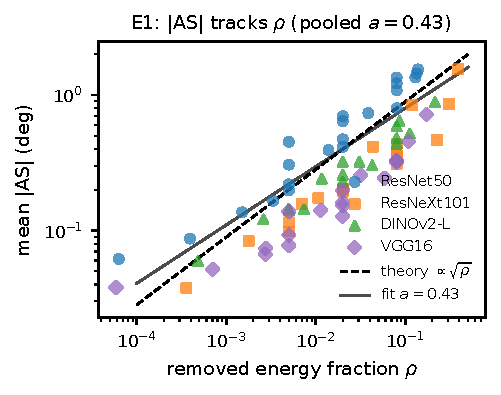
\includegraphics[width=\linewidth]{figs/fig_e1_energy.pdf}
\vspace{-0.4em}
\caption{E1 cells: $|$AS$|$ vs.\ $\rho$. Dashed: $\sqrt{\rho}$ theory; solid: fitted $a{=}0.43$.}
\label{fig:e1}
\vspace{-0.6em}
\end{figure}

High/low energy ratios at fixed $d$ exceed $3\times$ on all 4 evaluable models (e.g.\ ResNet $11$--$22\times$, ResNeXt $\approx10\times$, DINOv2 $3.7$--$5.1\times$, VGG16 $6$--$10\times$).
Fixed-$\rho$ max/min across $d$ still exceeds $1.5$ on several cells (ResNet up to $2.29$ at $\rho{=}0.5\%$).
EVA02-L ($d_{\mathrm{null}}{=}24$) is not evaluable beyond its full-null cell.
Energy dominates the fit and comes within $\approx0.07$ of the $\sqrt{\rho}$ exponent from the geometry argument above. At the same time, AS still varies with $d$ at fixed $\rho$, so the pre-registered ENERGY-DRIVEN flatness rule is only partly met. We treat the E1 outcome as mixed.

\section{A size-fair score}
\vspace{-0.2em}
Take an energy-matched random baseline: draw a Haar subspace of the full feature space that removes exactly the same energy $\mathbb{E}\|\Pi f\|^2$ as the null projector, and let $\mathrm{AS}_{\mathrm{rand}}$ be its mean $|$AS$|$ (20 draws).
Then
\[
\mathrm{AS}_{\mathrm{fair}} \;=\; \frac{\mathrm{AS}_{\mathrm{null}}}{\mathrm{AS}_{\mathrm{rand}}}.
\]
Values near $1$ mean the null shifts about as much as a random equal-energy subspace; values $\gg1$ mean the leakage is concentrated in the null.
This is the E3-registered definition, reused at $\alpha{=}0$ for the E2 audit.

\section{Planted leakage (E3)}
\vspace{-0.2em}
We plant a CLIP concept direction (\texttt{red}/\texttt{striped}/\texttt{water}) into each of 8 models' null spaces at log-uniform $\alpha\in[0.01,1]$ over 50 trials, leaving logits unchanged (max $|\Delta\mathrm{logit}|\le2.3{\times}10^{-5}$).
Kendall $\tau$ vs.\ the planted-$\alpha$ ranking, concept-averaged:
$\mathrm{AS}_{\mathrm{SING}}$ $0.386$ $[0.324,0.447]$;
$\mathrm{AS}_{\mathrm{fair}}$ $0.071$ $[0.004,0.138]$.
Neither recovers planted strength well; $\mathrm{AS}_{\mathrm{fair}}$ sits near chance.
Per-concept means look similar (red $0.386/0.070$, striped $0.403/0.061$, water $0.369/0.083$).
A few quirks: DeiT3-L signed AS is negative at every $\alpha$ and $|$AS$|$ shrinks as $\alpha$ grows; BiT $\mathrm{AS}_{\mathrm{SING}}$ reaches $17$--$20^\circ$ at $\alpha{=}1$ while its $\mathrm{AS}_{\mathrm{fair}}$ at $\alpha{=}0$ is only $0.045$--$0.063$; $\mathrm{AS}_{\mathrm{fair}}$ is non-monotonic in $\alpha$ for EVA02-L and ConvNeXt-B.
Correcting for size and recovering a planted ranking are different goals, and the two scores trade off between them.
We propose $\mathrm{AS}_{\mathrm{fair}}$ only as a size correction for cross-model AS comparisons. It is not meant as a calibrated leakage oracle.

\section{Audit of SING's 13-model claims (E2)}
\vspace{-0.2em}
On the same 10k subset plus a 200-image claim-class set (all 50 val images of jellyfish, porcupine, Arabian camel, sports car), we recompute $\mathrm{AS}_{\mathrm{SING}}$ and $\mathrm{AS}_{\mathrm{fair}}$ for all 13 released translators.

\begin{figure}[t]
\centering
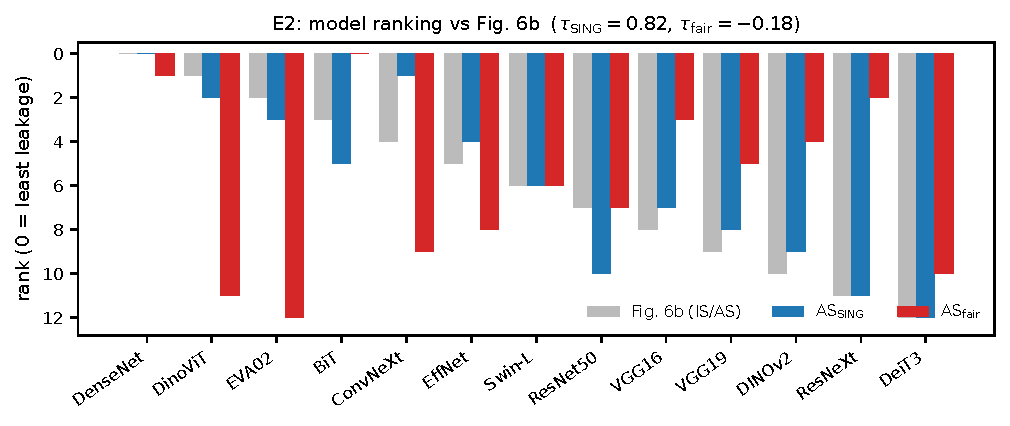
\includegraphics[width=\linewidth]{figs/fig_e2_ranking.pdf}
\vspace{-0.4em}
\caption{Ranks (0$=$least leakage). $\mathrm{AS}_{\mathrm{SING}}$ tracks Fig.~6b; $\mathrm{AS}_{\mathrm{fair}}$ does not.}
\label{fig:e2rank}
\vspace{-0.4em}
\end{figure}

\begin{figure}[t]
\centering
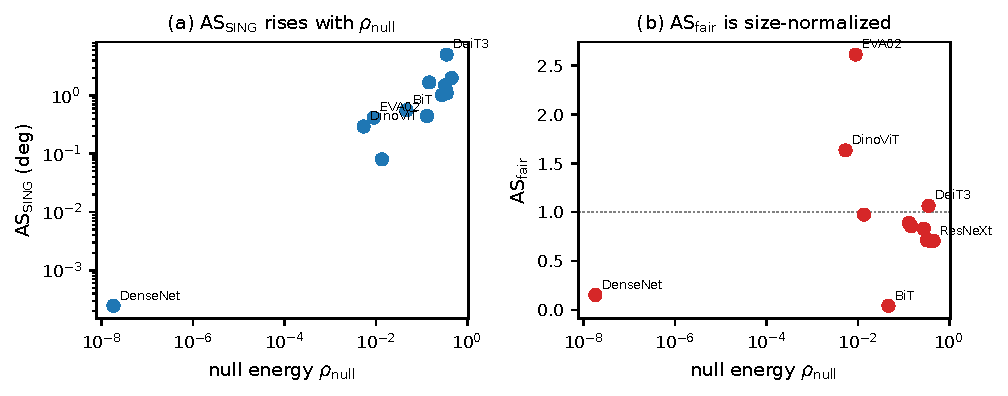
\includegraphics[width=\linewidth]{figs/fig_e2_scatter.pdf}
\vspace{-0.4em}
\caption{(a)~$\mathrm{AS}_{\mathrm{SING}}$ rises with $\rho_{\mathrm{null}}$. (b)~$\mathrm{AS}_{\mathrm{fair}}$ removes that trend.}
\label{fig:e2sc}
\vspace{-0.6em}
\end{figure}

\paragraph{Ranking.}
Against the digitized Fig.~6b IS/AS order:
$\tau(\mathrm{AS}_{\mathrm{SING}}){=}0.821$ ($p{=}1.3{\times}10^{-5}$);
$\tau(\mathrm{AS}_{\mathrm{fair}}){=}{-}0.179$ ($p{=}0.435$).
Dropping DenseNet: $\tau(\mathrm{AS}_{\mathrm{fair}}){=}{-}0.364$.
Mean over 173 SING concepts: $\tau{=}0.641$ vs.\ $-0.026$.
$\mathrm{AS}_{\mathrm{SING}}$ recovers SING; the disagreement shows up only after the size correction (Figs.~\ref{fig:e2rank}--\ref{fig:e2sc}).

\paragraph{Claim reversals.}
Under $\mathrm{AS}_{\mathrm{fair}}$, claims C1--C7, C9, C11, C12 reverse relative to $\mathrm{AS}_{\mathrm{SING}}$ (DinoViT is no longer least leaky; ResNeXt is no longer among the worst).
Two claims reverse under \emph{both} scores, with bootstrap CIs:
\begin{itemize}
\item \textbf{C8} (ResNet porcupine / sports-car $\ge$90th percentile): porcupine percentile $84.8$ $[80.1,87.7]$ ($\mathrm{AS}_{\mathrm{SING}}$), $68.4$ $[64.5,71.5]$ ($\mathrm{AS}_{\mathrm{fair}}$); sports car $61.0$ $[56.1,66.2]$ and $67.2$ $[63.6,71.4]$.
\item \textbf{C10} (DinoViT jellyfish $\gg$ camel): jellyfish$-$camel CI $[{-}0.205,{-}0.010]$ ($\mathrm{AS}_{\mathrm{SING}}$) and $[{-}1.403,{-}0.458]$ ($\mathrm{AS}_{\mathrm{fair}}$)---opposite in sign to SING's claim.
\end{itemize}

\paragraph{Caveats.}
(i)~C1/C2 are IS/AS-ratio claims tested here on $|$AS$|$; C11 is a steering claim proxied by null-removal AS; C10 uses class-text AS on 50 images/class (SING used $\approx$30 concepts / $\approx$1300 images).
(ii)~DenseNet has $\rho_{\mathrm{null}}{=}1.8{\times}10^{-8}$, so $\mathrm{AS}_{\mathrm{fair}}$ is degenerate.
(iii)~C13 (EVA02 as target space) is untestable: no EVA02-space translators were released.
(iv)~Our DinoViT IS/$|$AS$|$ is $20.95$ vs.\ $70.16$ in Fig.~6b---absolute ratios differ, but the $\mathrm{AS}_{\mathrm{SING}}$ ranking still agrees.

\begin{table}[t]
\centering
\scriptsize
\setlength{\tabcolsep}{2.5pt}
\begin{tabular}{@{}clcc@{}}
\toprule
ID & Claim (short) & $\mathrm{AS}_{\mathrm{SING}}$ & $\mathrm{AS}_{\mathrm{fair}}$ \\
\midrule
C1 & DinoViT best IS/AS among 5 & holds & reverses \\
C2 & ResNeXt lowest IS/AS among 5 & holds & reverses \\
C3 & ResNet leaks more than DinoViT & holds & reverses \\
C4 & DinoViT least class leakage & holds & reverses \\
C5 & ResNeXt high AS (top-2 of 5) & holds & reverses \\
C6 & ResNet per-class AS $>$ DinoViT & holds & reverses \\
C7 & DinoViT per-class $|$AS$|{<}1$ & holds & reverses \\
C8 & Porcupine/sports-car $\ge$90th pct. & reverses & reverses \\
C9 & No ResNet--DinoViT class corr. & holds & reverses \\
C10 & Jellyfish $\gg$ camel (DinoViT) & reverses & reverses \\
C11 & DinoViT least steerable (proxy) & holds & reverses \\
C12 & Fig.~6b 13-model order & holds & reverses \\
C13 & EVA02 target-space order & untestable & untestable \\
\bottomrule
\end{tabular}
\vspace{-0.4em}
\caption{E2 claim audit. C1/C2/C11 use $|$AS$|$ proxies; C10 is class-text on 50 imgs/class.}
\label{tab:claims}
\vspace{-0.8em}
\end{table}

Under $\mathrm{AS}_{\mathrm{fair}}$, DinoViT sits near the \emph{worst} end (12th of 13 by class $\mathrm{AS}_{\mathrm{fair}}$; EVA02 worst); under $\mathrm{AS}_{\mathrm{SING}}$ it ranks 3rd.
BiT becomes best under $\mathrm{AS}_{\mathrm{fair}}$ ($0.042$) because random subspaces of matched energy already move AS by $13.2^\circ$---the same translator-cancellation regime as Exp~1.
DenseNet's near-zero $\rho$ makes $\mathrm{AS}_{\mathrm{fair}}$ numerically unstable, so we also report $\tau$ without it (${-}0.364$).

\section{Discussion}
\vspace{-0.2em}
SING's within-model AS is a useful probe of translator-mediated null content. Used across models, it conflates semantics with how large and energetic the null is.
A boring baseline already said as much: over 13 models, Spearman$(\rho_{\mathrm{full}},|$AS$|_{\mathrm{full}}){=}0.87$ and Spearman$(\rho_{\mathrm{full}},\mathrm{IS}/\mathrm{AS}){=}{-}0.94$.
On top of that, the DinoViT label has no public checkpoint behind it.

\paragraph{Role of $\mathrm{AS}_{\mathrm{fair}}$.}
It divides null AS by an energy-matched random baseline so models are not rewarded for a small or low-energy null.
E3 shows that neither score recovers planted $\alpha$ rankings at the pre-registered $\tau\ge0.8$ bar, and $\mathrm{AS}_{\mathrm{fair}}$ is worse at that particular task.
We do not claim any replacement score beyond this size correction.

\paragraph{Practical suggestions.}
For any null-space leakage comparison:
\begin{enumerate}
\item Name the exact checkpoint and measured top-1 (avoid unverifiable labels such as ``DinoViT'').
\item Report $d_{\mathrm{null}}$ and $\rho_{\mathrm{null}}$ next to the score.
\item Report $\mathrm{AS}_{\mathrm{fair}}$ (or another energy-matched baseline) beside raw AS.
\item Flag translator condition numbers when full-null and block-wise AS disagree (BiT).
\item Prefer within-model interventions (subspace size, planted signal) over cross-architecture league tables when $d$ and $\rho$ vary widely.
\end{enumerate}

\paragraph{Limitations.}
On energy vs.\ dimension, E1 leaves the question partly open.
E3 shows $\mathrm{AS}_{\mathrm{fair}}$ does not recover planted $\alpha$.
Several E2 claims use proxies (C1/C2/C10/C11); DenseNet's $\mathrm{AS}_{\mathrm{fair}}$ is degenerate; C13 is untestable.
ImageNet-derived features restrict redistribution.
We did not retrain translators, evaluate a true DINO ViT-B/16~\citep{dino2021}, or extend the size audit to ViM~\citep{vim2022} / Cook~\citep{cook2020} / Rezaei~\citep{rezaei2023} scores~\citep{makonnen2025}.

\section{Conclusion}
\vspace{-0.2em}
SING's AS ranking of 13 classifiers reproduces with the released translators, but it is size-confounded. Correcting for null energy with $\mathrm{AS}_{\mathrm{fair}}$ breaks the published order ($\tau{:}\,0.82\to{-}0.18$) and reverses multiple claims, and the ``DinoViT'' result cannot be pinned on DINO.
Until a calibrated leakage oracle exists, cross-model null-space comparisons should report $\rho$ and a size-fair baseline alongside raw AS.

\vspace{0.4em}
\noindent\textbf{Reproducibility.}
Analysis code and aggregated tables: \url{https://github.com/sudeshgm/ic014-sing-null-dimension}.
ImageNet features are private.

{\small
\bibliographystyle{plainnat}
\bibliography{refs}
}

\appendix
\section{Additional numerical detail}
\vspace{-0.2em}
\paragraph{Exp~1 full-null anchors.}
Mean $|$AS$|$ at full null: ResNet50 $1.682^\circ$, ResNeXt101 $1.999^\circ$, BiT $0.556^\circ$, DINOv2-L $1.499^\circ$; at $d{=}24$: $0.166$, $0.175$, $9.30$, $0.143$ (seed SD in RESULTS.md).

\paragraph{E2 per-model class scores.}
Table~\ref{tab:e2models} lists $\rho_{\mathrm{null}}$, $\mathrm{AS}_{\mathrm{SING}}$, $\mathrm{AS}_{\mathrm{rand}}$ and $\mathrm{AS}_{\mathrm{fair}}$ used for the ranking.

\begin{table}[h]
\centering
\scriptsize
\setlength{\tabcolsep}{2.5pt}
\begin{tabular}{@{}lrrrr@{}}
\toprule
Model & $\rho_{\mathrm{null}}$ & AS$_{\mathrm{SING}}$ & AS$_{\mathrm{rand}}$ & AS$_{\mathrm{fair}}$ \\
\midrule
VGG16       & 0.350 & 1.088 & 1.537 & 0.708 \\
VGG19       & 0.339 & 1.256 & 1.755 & 0.716 \\
DenseNet121 & 1.8e-8 & 0.00025 & 0.0016 & 0.152 \\
ResNet50    & 0.146 & 1.676 & 1.960 & 0.855 \\
DinoViT     & 0.0054 & 0.294 & 0.180 & 1.632 \\
EffNet-B0   & 0.130 & 0.443 & 0.498 & 0.889 \\
BiT-R50x1   & 0.046 & 0.557 & 13.24 & 0.042 \\
ResNeXt101  & 0.451 & 1.999 & 2.829 & 0.707 \\
ConvNeXt-B  & 0.0135 & 0.080 & 0.083 & 0.974 \\
Swin-L      & 0.274 & 1.019 & 1.229 & 0.829 \\
DINOv2-L    & 0.322 & 1.499 & 2.105 & 0.712 \\
DeiT3-L     & 0.348 & 5.048 & 4.738 & 1.065 \\
EVA02-L     & 0.0089 & 0.417 & 0.160 & 2.612 \\
\bottomrule
\end{tabular}
\vspace{-0.3em}
\caption{E2 class-text scores on the 10k subset (from \texttt{e2\_models.csv}).}
\label{tab:e2models}
\end{table}

\paragraph{E3 per-concept $\tau$.}
AS$_{\mathrm{SING}}$ / AS$_{\mathrm{fair}}$:
red $0.386$ / $0.070$;
striped $0.403$ / $0.061$;
water $0.369$ / $0.083$.

\end{document}
